
\chapter{Modeling influence on a Social Network using Interaction Characteristics}


\section{Introduction}
% no \IEEEPARstart
The importance of social networks has been realized since the advent of Facebook in 2004 as well as other social networks such as Twitter, Flickr and Instagram. When a user posts a message on social media, other users in the network respond to the content by performing certain actions which create cascading effects within the network and is visible in the form of further activity. The fact that a message from one user prompted certain reactions from other users is an indication of the influence of one user over others in the network. This can be used to enhance the visibility of a product, viral marketing, and spreading awareness or even during disasters to alert citizens, or spreading hatred or rumors. \\

It is due to this popularity social media analytics has attracted a lot of attention from the research communities in machine learning \cite{aps:1} \cite{aps:8} \cite{aps:4}, preference learning \cite{aps:9}, recommendation systems, data mining \cite{aps:10}, information retrieval \cite{aps:11} etc. Social networks belong to the category of networks called strategic network models where the relation between nodes is determined by the choice of the members involved, not by a random rule. This means that the characteristics of nodes are important in determining whether links shall be formed. This also decides whether the information that is diffused can reach more nodes of the network. Chen \textit{et. al} and Subbian \textit{et. al} have proposed methods for finding influential nodes which use the process of information diffusion or social capital to discover the nodes with high diffusion centrality \cite{aps:12} \cite{aps:13}. Holander \textit{et. al} have argued that use of Eigenvector centrality as a measure is insufficient in deciding the and ranking influential nodes in online networks \cite{aps:15} \cite{aps:14}. \\

Influence maximization problem is a NP hard problem of identifying the subset of nodes in a social network that would maximize the coverage of information in the graph through diffusion. However the problem of assigning influence scores to every node in the graph is different compared to Influence Maximization since the former is a measurement problem, while the latter is a subset selection problem and both have different objectives \cite{aps:12} \cite{aps:13}. In influence ranking, Klout rank proposed by Rao \textit{et al}. has achieved significant breakthrough in calculating the current influence or rank of the user in the social network by analyzing the interaction characteristics generated by the user on a social network in the preceding 90 days \cite{aps:14}. The mathematical model implemented to calculate the Klout rank uses a feature vector of 3600 attributes.  The parameters of the model have been tuned by analyzing 45 billion interactions of various users collected from online networks. Machine learning techniques applied on data to create a predictive model has been investigated by Alexy \textit{et al}. \cite{aps:19} \cite{aps:17}. The model uses interaction characteristics such as number of mentions over time to create a PageRank like score for ranking users by their influence. Behnam \textit{et al}. \cite{aps:18} modeled influence using metrics such as number of followers and their ratio of affection to a particular topic. However previous literature ignored making up decision rules and understanding complex relationships between features that could lead to development of an objective criteria for calculating and comparing influence.\\


In this paper, attributes that are accumulated by the behavior of a person on the social network are used. The key assumption is that these attributes have a relationship with the influence of the person and can be used to create a feature vector to model the influence. The online characteristics that can be measured by information extracted from an online social network are impressions, clicks, likes, comments, re-shares, followers. Such attributes are difficult to emulate or artificially enhance and hence are appropriate indicators for developing an objective criteria for assessing the influence.\\

We have conducted experiments on the real world dataset from twitter to validate the effectiveness of the proposed approach. \\

The highlights of the paper are summarized as follows :\\

\begin{enumerate}
  \item A machine learning approach to study the comparison of influencers in the social network using various algorithms and their effectiveness on the data.
  \item Analysis of various features and their use in training and building a model.
        \item Use of feature selection, feature ranking techniques and their effect on the model and the predictions. Thus obtaining a smaller set of predictors that decide influence within a network.
        \item Validation of the model and comparisons to establish which of the techniques has best results. 
        \\
\end{enumerate}
	

Section II presents the related work in the field and the introduction to machine learning models and other techniques implemented in the paper. Section III formulates the problem, provides the objective function and then proposed approach. Section IV provides information about the data set, the methodology, experimental design and results. The conclusion is given in Section V.

\section{Related Work}

\subsection{Twitterrank: finding topic-sensitive influential twitterers}
The TwitterRank algorithm was implemented for studying people who are the most influential in the social network. The algorithm is based on the hypothesis that the measure of influence of a person is related to both the topical similarity between twitterers and the link structure. The authors argue that they could find evidence to support the theory which states that more followers a person has in a social network the more is the influence i.e. in-degree of a node is proportional to its influence in the network. The algorithm works on the assumption that there exists homophily within twitter i.e. same interests decide the relationship between the users. However no correlation is presented in the form of a degree distribution to prove existence of homophily \cite{aps:20} \cite{aps:16}. 


\subsection{Finding influencers using social capital}
The concept of “social capital” is proposed by the authors. According to them "Social capital" is computed by means of bonding and bridging capital. The bonding capital is defined as the ability to calibrate similar people against each other. The bridging capital is defined as the ability to connect diverse people. A bridging node is like an interdisciplinary researcher who connects different communities of researchers and a bonding node is a good researcher in a domain. It is argued that such nodes create a value throughout the network and this value is shared by them. The hypothesis is that this value is proportional to the influence of the node amongst other nodes it is connected to in the network. The social capital and its distribution amongst the nodes is based on the concept of distance based utility which is seen in strategic network formation process. The distance-based utility concept assumes that all players (nodes) have a utility in the network that is alike. Furthermore it takes into account only the benefits that a node in the network derives from other nodes to which it has indirect links. For the purpose of computing the value derived through the indirect links only links having minimum path length from source to destination are considered. These two features are considered as drawbacks of the distance-based utility in general and the same have been seen in the social capital based approach \cite{aps:13}.

\subsection{Geo-social Influence Spanning Maximization}
The Influence maximization problem has been modified to include the physical location of the social users in an attempt to solve the NP- Hard problem of identifying a small set of users that can influence the maximum number of users in a network. The technique measures influence as a factor of diffusion potential of a node. It is computationally expensive and may yield results that cannot guarantee global optimal solution due to the vast search space. The technique proposed uses greedy algorithm to identify the top "k" seeds that can propagate the influence across the network. The technique also proposes a hybrid indexing structure OIR*- tree which combines the features of an ordered influential user list and R*-tree. The indexing structure doesn’t consider the changing in the influence with time. The space complexity of this approach is higher as the influential nodes have to be stored. This approach is not useful for measuring influence of the node in a network \cite{aps:21}.

\subsection{Mining Time-Dependent Influential Users in Facebook Fans Group}
"Klout rank" is a popular method of using machine learning techniques to calculate the influence of a user in a network. The klout score is computed based on the statistics calculated about the user from various social platforms and a score is assigned to them. The technique however doesn’t consider that influence is time dependent. This means that a user may not have a high average klout score but could be influential at a particular time period. Klout also works on a “black box” model that doesn’t explain what can affect the influence of users in a network. Bias/variance graphs are not presented to indicate whether having 3600 features can lead to overfitting \cite{aps:23} \cite{aps:22}.


% An example of a floating figure using the graphicx package.
% Note that \label must occur AFTER (or within) \caption.
% For figures, \caption should occur after the \includegraphics.
% Note that IEEEtran v1.7 and later has special internal code that
% is designed to preserve the operation of \label within \caption
% even when the captionsoff option is in effect. However, because
% of issues like this, it may be the safest practice to put all your
% \label just after \caption rather than within \caption{}.
%
% Reminder: the "draftcls" or "draftclsnofoot", not "draft", class
% option should be used if it is desired that the figures are to be
% displayed while in draft mode.
%
%\begin{figure}[!t]
%\centering
%\includegraphics[width=2.5in]{myfigure}
% where an .eps filename suffix will be assumed under latex, 
% and a .pdf suffix will be assumed for pdflatex; or what has been declared
% via \DeclareGraphicsExtensions.
%\caption{Simulation results for the network.}
%\label{fig_sim}
%\end{figure}

% Note that the IEEE typically puts floats only at the top, even when this
% results in a large percentage of a column being occupied by floats.


% An example of a double column floating figure using two subfigures.
% (The subfig.sty package must be loaded for this to work.)
% The subfigure \label commands are set within each subfloat command,
% and the \label for the overall figure must come after \caption.
% \hfil is used as a separator to get equal spacing.
% Watch out that the combined width of all the subfigures on a 
% line do not exceed the text width or a line break will occur.
%
%\begin{figure*}[!t]
%\centering
%\subfloat[Case I]{\includegraphics[width=2.5in]{box}%
%\label{fig_first_case}}
%\hfil
%\subfloat[Case II]{\includegraphics[width=2.5in]{box}%
%\label{fig_second_case}}
%\caption{Simulation results for the network.}
%\label{fig_sim}
%\end{figure*}
%
% Note that often IEEE papers with subfigures do not employ subfigure
% captions (using the optional argument to \subfloat[]), but instead will
% reference/describe all of them (a), (b), etc., within the main caption.
% Be aware that for subfig.sty to generate the (a), (b), etc., subfigure
% labels, the optional argument to \subfloat must be present. If a
% subcaption is not desired, just leave its contents blank,
% e.g., \subfloat[].


% An example of a floating table. Note that, for IEEE style tables, the
% \caption command should come BEFORE the table and, given that table
% captions serve much like titles, are usually capitalized except for words
% such as a, an, and, as, at, but, by, for, in, nor, of, on, or, the, to
% and up, which are usually not capitalized unless they are the first or
% last word of the caption. Table text will default to \footnotesize as
% the IEEE normally uses this smaller font for tables.
% The \label must come after \caption as always.
%
%\begin{table}[!t]
%% increase table row spacing, adjust to taste
%\renewcommand{\arraystretch}{1.3}
% if using array.sty, it might be a good idea to tweak the value of
% \extrarowheight as needed to properly center the text within the cells
%\caption{An Example of a Table}
%\label{table_example}
%\centering
%% Some packages, such as MDW tools, offer better commands for making tables
%% than the plain LaTeX2e tabular which is used here.
%\begin{tabular}{|c||c|}
%\hline
%One & Two\\
%\hline
%Three & Four\\
%\hline
%\end{tabular}
%\end{table}


% Note that the IEEE does not put floats in the very first column
% - or typically anywhere on the first page for that matter. Also,
% in-text middle ("here") positioning is typically not used, but it
% is allowed and encouraged for Computer Society conferences (but
% not Computer Society journals). Most IEEE journals/conferences use
% top floats exclusively. 
% Note that, LaTeX2e, unlike IEEE journals/conferences, places
% footnotes above bottom floats. This can be corrected via the
% \fnbelowfloat command of the stfloats package.

\section{Mathematical Model}
An online social network is represented as a graph G = (V, E) with nodes (V) represents the number of users and edges (E) denote friendship between two users. In most of the social networks the users send requests to other users to form a relationship. The acceptance of this request is then a undirected link. Usually the friendhsip links in a social networking graph can be both undirected (Facebook) as well as directed (Twitter). The nodes also have properties that are due to the membership of this network. These properties are derived from membership of the network and are varied by the influence of his behavior on the network and the networks influence on his behavior i.e. co-evolution.  \\

The measurement problem of calculating the influence shall become a problem of supervised learning. Supervised learning algorithms are of many types and there is no single algorithm that can work on any given supervised learning problems. Neural networks perform well if the task involves identifying complex set of dependencies and identifying these dependencies. However the best configuration of a neural network has to be determined experimentally.\\


\subsection{Calculation of Influence Score}
A feature vector $x_i$ is constructed for each user from the set of features extracted for each user from Twitter as shown in Table 1. Then a Given a set of N training examples of the form {($x_1$, $y_1$), …, ($x_n$, $y_n$)} such that $x_i$ is the feature vector of the $i^{th}$ example and $y_i$ is its class label. The algorithm creates a function $g: X \rightarrow Y$ where X is the input space and Y is the output space.

\begin{table}[!h]
\renewcommand{\arraystretch}{1.3}
\caption{Feature vector}
\label{table}
\centering
\begin{tabular}{|c|c|c|c|}
  \hline
\multicolumn{1}{|c|}{\textbf{Sr. No}} & \multicolumn{1}{c|}{\textbf{Feature list}} & \multicolumn{1}{c|}{\textbf{Sr. No}} & \multicolumn{1}{c|}{\textbf{Feature list}}\\
  \hline
  1 & Follower count & 5 & Following count\\
  \hline
  2 & Listed count & 6 & mentions received\\
  \hline
  3 & retweets received & 7 & mentions received\\
  \hline
  4 &  retweets sent & 8 & posts\\
  \hline
\end{tabular}
\end{table}

\subsection{Model Representation}

\subsubsection{Artificial Neural Networks}
Artificial neural networks are composed of input layers, hidden layers and output layers. The number of hidden layers ideally should be more as they can compute more nonlinear relationships between the inputs. However, it is important to avoid over-fitting while deciding the number of hidden layers and the number of hidden units. The input feature matrix $X$ and the weight matrix of the $W_{21}$ $(\theta_{1})$ and the result are given to the sigmoid function to decide which neurons of the hidden layer 1 i.e. ($a_{1}$) are activated. The output of this hidden layer is the multiplied with the second weight matrix $W_{31}$ $(\theta_{2})$ and so on till the output layer. The back-propagation algorithm is then used to obtain the adjusted weights. The cost function of the network for the classification problem is provided in Eqn. (1) and the penalty term (regularization) is used to it for preventing over-fitting is provided in Eqn.(2).\\


\begin{figure}
\centering
\fbox{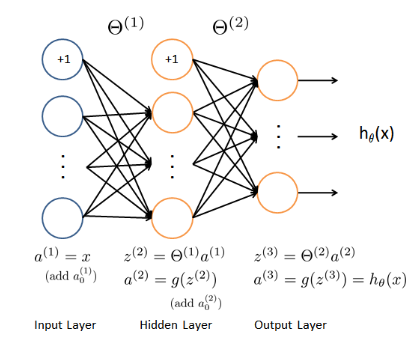
\includegraphics[scale=0.45]{fignn.png}}
\caption{Neural Network Architecture with Backpropagation}
\label{fig 1}
\end{figure}



\subsubsection{Cost Function - Artificial Neural Networks}

The cost function is that of the standard regularized logistic regression which is generalized for $k$ outputs instead of one output. For our problem the output is a single value of 0/1 depending upon whose influence in a network is more. The cost function shall be minimized using the back propagation algorithm to get the ideal value of the weights.

\begin{equation}
J(\Theta ) = \frac{a}{b} \sum_{i=1}^{k}\sum_{k=1}^{k} * [-y_{k}^{i}*log((h_{\Theta }(x^{i}))_{k}) - (1-y_{k}^{(i)})*log((h_{\Theta }(x^{i}))_{k})] 
\end{equation}
\begin{equation}
Penalty =  \frac{\lambda }{m}* [\sum_{j=1}^{J1}\sum_{k=1}^{K1}*(\Theta _{(j,k))}^{(1))})^{2} + \sum_{j=1}^{J2}\sum_{k=1}^{K2}*(\Theta _{(j,k))}^{(2))})^{2}]
\end{equation}

\subsubsection{Gradient boosted trees}

Gradient boosting is a technique that combines several weak learners into a strong learner using multiple iterations. Gradient boosting is applied with decision trees of fixed size as the first level learners. The decision tree partitions the input space into disjoint regions and predicts a constant value in each region. The General idea for a gradient boosted tree is to fit a model to the data i.e $F_1$(x) = y . Fit the model to the residuals denoted by $h_{(1)(x)}$ = y - $F_1$(x). Then obtain a new model $F_2$(x) = $F_1$(x) + $h_1$(x). The value of 'm' or the hyper parameter which gives the number of iterations of the residual correction procedure is obtained by cross validation. \\ 





\subsubsection{Gradient Boosted trees}



Model Update rule:

\begin{equation}
F_{m}(x) = F_{(m-1)}(x)) + \sum_{j=1}^{J_m} \gamma_{jm} I (x \epsilon R_{jm}) 
\end{equation}

\subsection{Influence Ranking Algorithm}

The algorithm for comparison of influence between two users whose network features have been collected from Twitter is presented. The parameters of various models are set initially and these values are modified till the ideal values are obtained. The cross validation set is used for this purpose.\\

\begin{algorithm}
\caption{Influencer Ranking model}
\begin{algorithmic}[1]
 \State Set initial seed for random numbers
 \State Set the training control values
 \State Set the tuning grid for parameter search
 \For {each parameter set} do
 \For {each resampling iteration set} do
 \State hold out specific samples
 \State Pre process the data (Center and Scale)
 \State Fit the model on the remaining samples
 \State Predict the held out samples
 
 \EndFor
 \State Calculate the average performance across held out predictions
 \EndFor
 \State Determine the optimal parameter set
 \State Fit the final model to all the training data using optimal parameter set 
 

\end{algorithmic}
\end{algorithm}

\section{Experimental Study}

\subsection{Experiment setting}

The performance of the Influence Ranking algorithm in Section III-(C) is studied to understand the best set of features to measure influence.\\

\subsubsection{Dataset}  
The dataset comprises a standard, pair-wise preference learning task. Each data point describes two individuals whose identities are anonymized and their future references in the paper are made using labels 'A' and 'B'. For each person, 8 pre-computed, non-negative numeric features based on twitter activity are provided. The binary label represents a human judgement about which one of the two individuals is more influential. The Ground truth labels provided are 0/1 to indicate which of the users is more influential. The test set has 5952 entries for which label has to be predicted.

\begin{table}[!h]
\renewcommand{\arraystretch}{1.3}
\caption{Description of the dataset}
\label{table}
\centering
\begin{tabular}{|c|c|c|c|}
  \hline
\multicolumn{1}{|c|}{\textbf{Training set size}} & \multicolumn{1}{c|}{\textbf{Test set size}} & \multicolumn{1}{c|}{\textbf{Feature vector}} & \multicolumn{1}{c|}{\textbf{Classification}}\\
  \hline
  5500 & 5952 &  22 & Binary\\
  \hline
\end{tabular}
\end{table}


\subsection{Results}

The accuracy and performance on test set was measured for the Three layered ANN trained using correlated and uncorrelated predictors.

\begin{table}[H]
\renewcommand{\arraystretch}{1.3}
\caption{Modeling influence using Multilayered Perceptron with Backpropagation}
\label{table}
\centering
\begin{tabular}{|c|c|c|c|}
%\begin{tabular}{|p{0.1in}|p{0.75in}|p{0.51in}|p{.51in}|p{0.51in}|}
  \hline
\multicolumn{1}{|c|}{\textbf{Sample size}} & \multicolumn{1}{c|}{\textbf{Hidden units}} & \multicolumn{1}{c|}{\textbf{Training Accuracy}} & \multicolumn{1}{c|}{\textbf{Training Kappa}}\\
  \hline
  3521 &  16 & 72.29 & 44.55\\
  \hline
  3521 &  24 & 71.29 & 43.42\\
  \hline
  3521 &  32 & 71.55 & 43.04\\
  \hline
\end{tabular}
\end{table}

For above experiment correlated features ($\geq{0.75}$) were removed. Cross validation technique used was X-cross fold with X = 5 and 5 times repeat. Training set accuracy was used as selection criteria for evaluation and hidden units were decided as 16. The trained model gave an accuracy of 0.801 on the test set.


\begin{table}[!h]
\renewcommand{\arraystretch}{1.3}
\caption{Modeling influence using Multilayered Perceptron with Backpropagation}
\label{table}
\centering
\begin{tabular}{|c|c|c|c|}
  \hline
\multicolumn{1}{|c|}{\textbf{Sample size}} & \multicolumn{1}{c|}{\textbf{Hidden units}} & \multicolumn{1}{c|}{\textbf{Training Accuracy}} & \multicolumn{1}{c|}{\textbf{Training Kappa}}\\
  \hline
  3521 &  22 & 73.11 & 46.19\\
  \hline
  3521 &  33 & 72.96 & 45.89\\
  \hline
  3521 &  44 & 73.08 & 46.14\\
  \hline
\end{tabular}
\end{table}


For above experiment correlated features were allowed for training. Cross validation technique used was X-cross fold with X = 5 and 5 times repeat. Training set accuracy was used as selection criteria for evaluation and hidden units were decided as 22. The trained model with 22 hidden nodes gave accuracy of 0.81 on test set.

\begin{figure}[!h]
\centering
\fbox{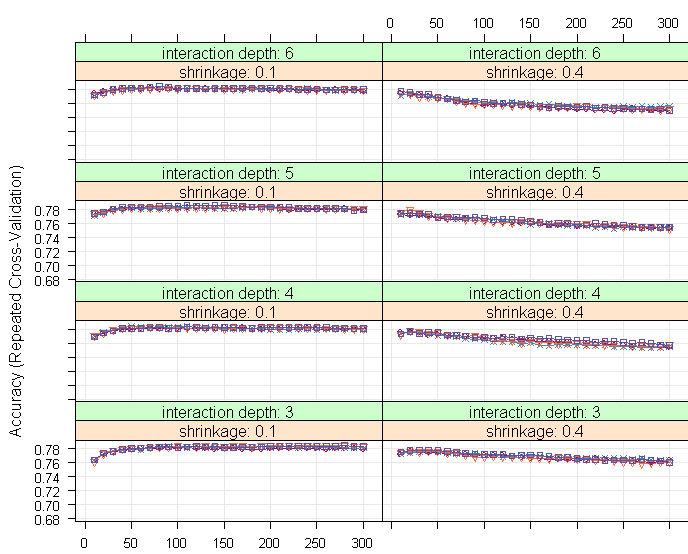
\includegraphics[scale=0.6]{figgbm.png}}
\caption{Performance of Gradient Boosted Trees}
\label{fig 1}
\end{figure}

Modeling influence using Decision trees with gradient boosting was performed. To tune the parameters of the trees such as Number of Trees $N_{trees}$, Shrinkage, Interaction depth and Minimum observations in nodes, a grid search was conducted. Training set Accuracy was the criteria to select the optimal model. Fig. 2 shows the performance of the algorithm during grid search and the accuracy is seen in Fig. 2 to degrade as the interaction depth increases beyond 5 and the shrinkage is increased beyond 0.1.  The final parameter values for the optimal model obtained through grid search were $N_{trees}$ = 110, interaction depth = 5, shrinkage = 0.1 and minimum observations in nodes = 20. The accuracy obtained on the test set was 0.8601.\\

Random forests (Rf) technique to model influence using the correlated features and removing correlation was performed. Advantage of random forests models are better accuracy but at the cost of interpret-ability of the model. The tuning parameter is Number of trees for these model whose value has to be determined empirically. The final model selected using training set accuracy had classification accuracy of 0.856 on the test set. The model with correlated features gave slightly better result 0.859. Removing correlation doesn’t improve accuracy on this dataset for the ANN and Rf.\\

Improving accuracy using ensembling, boosting or bagging at the cost of interpret-ability is a disadvantage for implementation. Such techniques have improved accuracy but such models obtained had more theoretical importance than practical value as seen in the NetFlix competition. Table V contains the training set and test set accuracy of greedy ensembles of GBM Trees, Random forests and ANN obtained in Section IV-B. The test set accuracy of the models is used as the selection criteria and Extreme Gradient Boosting has the highest accuracy on the test set at 0.87. ROC curves to denote the performance of Ensembled models of ANN, GBM, Rf is shown in Fig 3 and Area under curve is used as the selection criteria to obtain the optimal model. The results are shown for each combination in Fig. 3. The correlation between the predictions of GBM and Rf is 0.88 and so their ensemble was discarded due to highly correlated predictions. The highest accuracy on the test set is seen for the ensemble of GBM and Rf as shown in Table V.  \\

\begin{table}[!h]
\renewcommand{\arraystretch}{2.5}
\caption{Ensembled Predictors}
\label{table}
\centering
\begin{tabular}{|c|c|c|c|}
  \hline
\multicolumn{1}{|c|}{\textbf{Sr. No}} & \multicolumn{1}{c|}{\textbf{Technique}} & \multicolumn{1}{c|}{\textbf{Training Accuracy}} & \multicolumn{1}{c|}{\textbf{Test set Accuracy}}\\
  \hline
  1 & Boosting &  0.7856 & 0.82 \\
  \hline
  2 & Greedy Ensemble (ANN,GBM,RF) &  0.86 & 0.867 \\
  \hline
  3 & Greedy Ensemble (GBM,RF) &  0.86 & 0.83 \\
    \hline
  4 & Averaging Predictors (GBM,RF) &  0.79 & 0.866 \\
    \hline
  5 & Extreme Gradient Boosting &  0.79 & 0.87 \\
  \hline
\end{tabular}
\end{table}






\begin{figure}[H]
\centering
\fbox{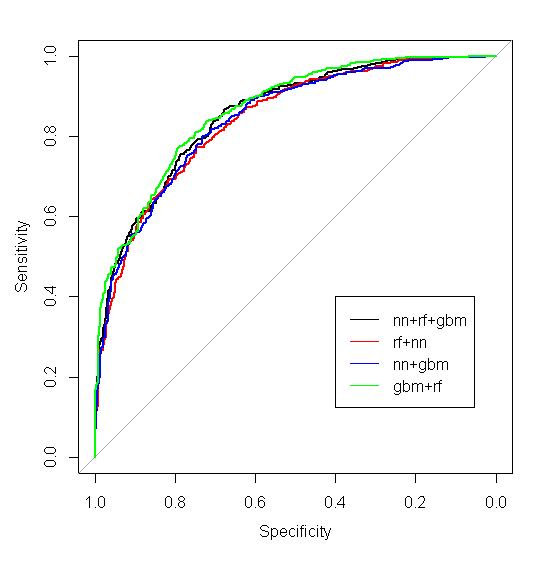
\includegraphics[scale=0.45]{figavg.png}}
\caption{Performance of Greedy Ensembles}
\label{fig 1}
\end{figure}



\section{Conclusion}
The framework for ranking influential nodes in a social network based on characteristics obtained from a nodes interaction on the social network has been presented in this paper. The influence is modeled using machine learning techniques unlike the conventional influence maximization approaches. Features of the individual nodes obtained from its interaction characteristics  are used and the network architecture is not considered. The performance metrics of the algorithms used in the experiments is classification accuracy and using this objective criteria Extreme Gradient Boosted decision tree has shown the highest accuracy. The influence ranking algorithm in this paper is a suitable technique for computation of the influence score of various nodes and this has been validated by the extensive experiments performed on Twitter dataset.  






